\documentclass{beamer}
\usepackage{listings}
\usepackage{multicol}
\usepackage[ruled,vlined]{algorithm2e} 
\usepackage{algpseudocode}


\lstset{
%language=C,
frame=single, 
breaklines=true,
columns=fullflexible
}
\graphicspath{./figures/}
\usepackage{subcaption}
\usepackage{url}
\usepackage{tikz}
\usepackage{tkz-euclide} % loads  TikZ and tkz-base
%\usetkzobj{all}
\usetikzlibrary{calc,math}
\usepackage{float}
\newcommand\norm[1]{\left\lVert#1\right\rVert}
\renewcommand{\vec}[1]{\mathbf{#1}}
\usepackage[export]{adjustbox}
\usepackage[utf8]{inputenc}
\usepackage{amsmath}
\providecommand{\pr}[1]{\ensuremath{\Pr\left(#1\right)}}
\providecommand{\brak}[1]{\ensuremath{\left(#1\right)}}
\providecommand{\cbrak}[1]{\ensuremath{\left\{#1\right\}}}
\providecommand{\sbrak}[1]{\ensuremath{\left[#1\right]}}
\usetheme{Boadilla}

\SetKwInput{KwInput}{Input}                % Set the Input
\SetKwInput{KwOutput}{Output}              % set the Output



\title{Research Paper Presentation}
\author{Ganesh Bombatkar-CS20BTECH11016}
\institute{}
\date{\today}
\begin{document}

\begin{frame}
\titlepage
\end{frame}

\begin{frame}{Title and Author}
    \begin{block}{Title}
    Estimation of Observation Error Probability in Wireless Sensor Networks
    \end{block}
    
    \begin{block}{Author}
    \begin{enumerate}
        \item Xin He
        \item Xiaobo Zhou
        \item Khoirul Anwar
        \item Tad Matsumoto 
    \end{enumerate}
    Advanced Institute of Science and Technology, Nomi, Ishikawa, Japan
    
    \end{block}
\end{frame}

\begin{frame}{Abstract}
    \begin{itemize}
        \item Propose for a parallel wireless sensor network (WSN) model
        \item A decoding technique that well exploits the knowledge of the sensing data to be transmitted from each sensor to the fusion center (FC).
        \item Algorithm to estimate the observation error probabilities
        \item The convergence of the algorithm is also evaluated with comparison of bit-error-rate (BER)
    \end{itemize}
\end{frame}

\section{System Model}
\begin{frame}{\textbf{System Model}}
    \begin{figure}
        \centering
        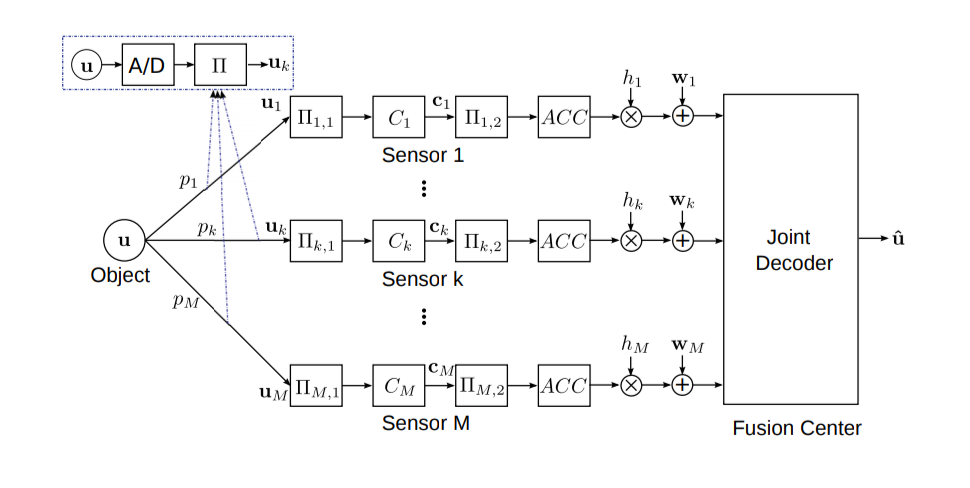
\includegraphics[scale=0.4]{figures/SystemModel.png}
        \caption{Structure of proposed system model}
        \label{fig:systemmodel}
    \end{figure}    
\end{frame}

\begin{frame}{\textbf{System Model}}
    \begin{enumerate}
    \setlength\itemsep{0.4em}
        \item \textit{A/D converter} : 
        \begin{itemize}
            \item convert analog signal to digital bit sequence
        \end{itemize}
        \item \textit{Interleaver} \brak{\mathbf{\Pi}} :
        \begin{itemize}
            \item Intermixes signal thus converting bunch error to random error
        \end{itemize}
        \item \textit{ Channel encoder} \brak{\mathbf{C_k}} :
        \begin{itemize}
            \item used to detect error and correct some of them
            \item Introduce bit sequence which help in overcoming effect of white noise
        \end{itemize}
        \item \textit{ACC} :
        \begin{itemize}
            \item Doped Accumulator (ACC) takes XOR of signal with some bit sequence
        \end{itemize}
        \item \textit{channel coefficient} :
        \begin{itemize}
            \item Scale a signal
        \end{itemize}
        \item \textit{White gaussion noise} :
        \begin{itemize}
            \item basic model to mimic effect of random process that occur in nature
        \end{itemize}
    \end{enumerate}
\end{frame}

\begin{frame}{\textbf{System Model}}
    \begin{itemize}
        \item Error corrupted binary sequence $u_k$ , $k$ $\in$ \cbrak{1,\dots,M} obtained after interleaver $\mathbf{\Pi}$ followed from A/D converter.
        \item $p_k$ be the bit flipping probability for the sensor $k$.
        \item signal $u_k$ is interleaved by $\mathbf{\Pi_{\text{K},1}}$ 
        \item Then encoded by channel encoder $C_k$ 
        \item encoded bit sequence $c_k$ interleaved by the interleaver $\mathbf{\Pi_{\text{k},2}}$ and doped-accumulated by ACC
        \item then it modulated by BPSK thus gives $s_k$
        \item transmitted to the FC over independent static AWGN channels
        \item finally we get bit sequence $y_k$
        \begin{align}
            y_k=h_k\times s_k + w_k 
        \end{align}
        $h_k$ is channel coefficient  and  $w_k$ is zero mean Gaussian noise
    \end{itemize}
\end{frame}

\section{Decoding}
\begin{frame}{\textbf{Decoding}}
    \begin{figure}
        \centering
        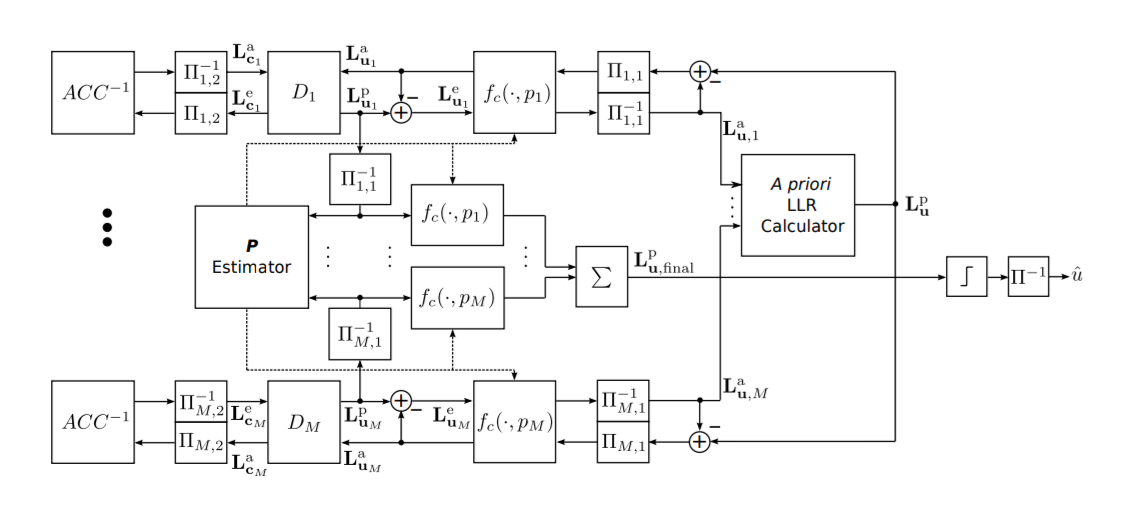
\includegraphics[scale=0.4]{figures/Decoder.png}
        \caption{ Proposed decoding strategy for a parallel sensor network}
        \label{fig:decoding}
    \end{figure}
\end{frame}

\begin{frame}{\textbf{Decoding}}
    Decoding consist of three parts :
    \begin{enumerate}
        \item Local iteration
        \begin{itemize}
            \item In LI extrinsic LLR exchange between decoder $D_k$ and doped accumulator $\mathbf{\text{ACC}^{-1}}$ takes place
            \item takes \textit{priori} LLR $\mathbf{L}^{a}_{\text{u}}$
            and gives back  \textit{posteriori} LLR $\mathbf{L}^{p}_{u k}$ after performing decoding and $\text{ACC}^{-1}$
        \end{itemize}
        \item P estimator
        \begin{itemize}
            \item then a \textit{posteriori} LLR $\mathbf{L}^{p}_{u k}$ containing some error are feed to P estimator to calculate $p_k$
            \item Value of $p_k$ are used by $f_c\brak{\cdot,p_k}$ function
        \end{itemize}
        \item Global iteration
        \begin{itemize}
            \item Extrinsic LLR exchange between Decoders
        \end{itemize}
    \end{enumerate}
    
    \textit{LI} and \textit{GI} are performed until no more relevant gain can be achieved in a final \textit{posteriori} LLR $\mathbf{L}^{p}_{\text{u,final}}$
\end{frame}


\section{P Estimation}
\begin{frame}{\textbf{P Estimation}}
      \begin{itemize}
        \item $ j = i + 1 \text{ if } i = 1 \dots M - 1 \quad \text{ and } j = 1 \text{ if } i = M$
        \item N : number of the LLR pairs with their absolute values larger than a given threshold T
    \end{itemize}
    \begin{align}
        \hat{q}_{i j}=\frac{1}{N}
        \sum_{1}^{N}
        \frac{
        \exp ({\mathbf{L}^{p}_{\text{u}i}})+\exp ({\mathbf{L}^{p}_{\text{u}j}})
        }
        {
        [{{1+\exp\brak{\mathbf{L}^{p}_{\text{u}i}}}}] \cdot [{1+\exp ({\mathbf{L}^{p}_{\text{uj}}})}]
        }
    \end{align}
    
  
    
    Let $\mathbf{I}$ be identity matrix of size $\mathbf{M}$   and $\mathbf{J}$ be defined in \eqref{J-matrix} of size $\mathbf{M}$
    \begin{align}
        \hat{\mathbf{q}}=\sbrak{\brak{\mathbf{I}+\mathbf{J}}-2\cdot \text{diag}\brak{\hat{\mathbf{P}}}\cdot\mathbf{ J}} \cdot \mathbf{\hat{P}}
    \end{align}
    Here $\mathbf{\hat{P}}=\sbrak{\hat{p}_1,\hat{p}_2,\dots,\hat{p}_M}^\mathbf{T}$ and $\mathbf{\hat{q}}=\sbrak{\hat{q}_{12},\hat{q}_{23},\dots,\hat{q}_{M1}}^\mathbf{T}$
  
    The diag($\cdot$) is the operator that forms a diagonal matrix from
its argument vector.
\end{frame}

\begin{frame}{\textbf{P Estimation}}
    \begin{align}
        \mathbf{J}=
        \begin{bmatrix}
            0 & 1 & 0 & 0 & \dots 0 \\
            0 & 0 & 1 & 0 & \dots 0 \\
            \vdots & \vdots & \vdots & \vdots & \vdots \\
            1 & 0 & 0 & 0 & \dots 0 
        \end{bmatrix}
        \label{J-matrix}
    \end{align}
    
    Objective : to find $\mathbf{\hat{P}} \succcurlyeq 0$ which minimize  
    $\mathbf{\Vert A\hat{{P}}-\hat{q} \Vert ^2}$
    \\ where, $\mathbf{A}=\sbrak{\mathbf{\brak{I+J}}-2\cdot \text{diag}\brak{\mathbf{\hat{P}}}\cdot \mathbf{J}}$
    
    We solve this using iterative algorithm summerized in Alogorithm 1.In this algorithm, we use the standard Non negative Least Squares \textit{(lsqnonneg) } algorithm
\end{frame}

\begin{frame}{}

\begin{algorithm}[H]
\SetAlgoLined
\KwInput{$\mathbf{\hat{q}}$, $\epsilon$, Pre-defined maximum iterations \textit{IT}$_m$}
\KwOutput{$\mathbf{\hat{P}}$ $\succcurlyeq$  0 such that  $\mathbf{\Vert A\hat{{P}}-\hat{q} \Vert ^2}$ is minimized}
 \textbf{Initialization:} $\mathbf{\hat{P}^{\brak{0}}=0,}$ Calculate $\mathbf{A}$ and $\mathbf{\Delta \brak{0}=}$ $\mathbf{\Vert A\hat{{P}}^{\brak{0}}-\hat{q} \Vert ^2}$ \;
\For{$l=1$ to \textit{IT}$_m$}{
Calculate $\mathbf{\hat{P}^{\brak{l}}}$ by using \textit{lsqnonneg} algorithm\;
 Update $\mathbf{A=\left[{\brak{I+J}-2\cdot \text{diag}\brak{\hat{P}^{(l)}}\cdot J}\right]}$\;
 $\mathbf{\Delta \brak{l}=\Vert A\hat{{P}}^{\brak{l}}-\hat{q} \Vert ^2}$\;
 \If{$\mathbf{\Delta \brak{l} > \Delta \brak{l-1}}$}{
 Exit For\;
 }
 \If{$\mathbf{\Vert \hat{{P}}^{\brak{l}} - \hat{{P}}^{\brak{l-1}} \Vert ^2\leq \epsilon}$}{
 Exit For\;
 }
}
$\mathbf{\hat{{P}}=\hat{{P}}^{\brak{l}}}$\;
 \caption{P Estimator}
\end{algorithm}

\end{frame}

\section{Significance}
\begin{frame}{\textbf{Significance}}
\begin{columns}[onlytextwidth]
    \column{0.7\textwidth}

    \begin{figure}
        \centering
        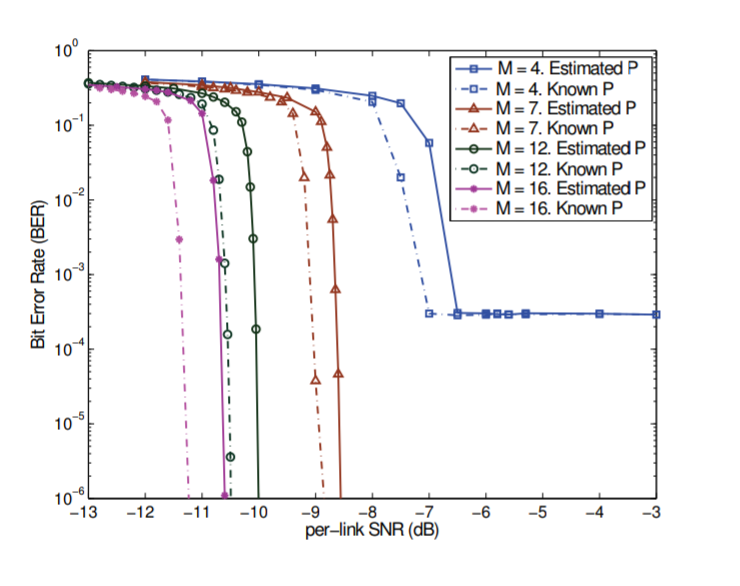
\includegraphics[scale=0.4]{figures/Ber-Performance.png}
        % \caption{Caption}
        \label{fig:berPerformance}
    \end{figure}
    
    \column{0.3\textwidth}
    Figure is drawn for 
    \begin{itemize}
        \item $\mathbf{T}=2$
        \item $\epsilon=10^{-6}$
        \item Iteration time \textit{IT}$_M$ $=20$
    \end{itemize} 

    \begin{block}{}
     using estimated $\mathbf{\hat{P}}$ can cause roughly $0.3 \text{to} 0.5$ dB loss in per-link SNR compared to actual $\mathbf{\hat{P}}$
    \end{block}
\end{columns}

\begin{block}{}
Our model gives $2 - 3 $ dB improvement than earlier models 
\end{block}
\end{frame}

\end{document}